\documentclass{article}

% Short communications of approximately 3000 words are also accepted. 
% These papers should contain no more than two figures, two tables, and thirty references. 
% A short abstract of fewer than 200 words is acceptable.

% Bibliography
\usepackage{natbib}
\bibpunct{(}{)}{;}{a}{}{;}

\usepackage[english]{babel}

% Use 'It was found that something is something (Name 1234)' style
\setcitestyle{authoryear,open={},close={}}

% Affiliations
\usepackage{authblk}
\title{The error when inferring phylogenies with incipient species by a Birth-Death model}
% \subtitle{Should protracted speciation be incorporated in phylogenetic tree construction methods?}

\author[1]{Rich\`el J.C. Bilderbeek}
\author[1]{Rampal S. Etienne}
\affil[1]{Groningen Institute for Evolutionary Life Sciences, University of Groningen, Groningen, The Netherlands}

% Use double spacing
\usepackage{setspace}
\doublespacing

\usepackage{pgf}
\usepackage{hyperref}
\usepackage{verbatim}
  
% Adds numbered lines
\usepackage{lineno}
\linenumbers

\begin{document}

\maketitle

\begin{abstract}

  % From 'How to construct a Nature summary paragraph'

  % A short abstract of fewer than 200 words is acceptable.

  % One or two sentences providing a basic
  % introduction to the field,
  % comprehensible to a scientist in any discipline.
  The tools for reconstructing phylogenetic relationships between taxonomic 
  units (e.g. species) have become very advanced in the last three decades. 

  % Two to three sentences of
  % more detailed background, comprehensible to
  % scientists in related disciplines.
  Among the most popular tools are Bayesian approaches, such as BEAST, MrBayes and RevBayes, 
  that use efficient tree sampling routines to create a posterior probability distribution 
  of the phylogenetic tree. 
  A feature of these approaches is the possibility to incorporate 
  known or hypothesized structure of the phylogenetic tree through the tree prior. 
  It has been shown that the effect of the prior on the posterior distribution 
  of trees can be substantial. 

  % One sentence clearly stating the general
  % problem being addressed by this particular
  % study.
  Currently implemented tree priors assume that speciation is instantaneous,
  where we know that speciation can be a gradual process.

  % One sentence summarising the main
  % result (with the words “here we show”
  % their equivalent).
  Here we explore the effects of ignoring 
  the protractedness of the speciation process with an extensive simulation study. 

  % Two or three sentences explaining what
  % the main result reveals in direct
  % comparison to what was thought to be the case
  % previously, or how the main result adds to
  % previous knowledge.

  % One or two sentences to put the results into a
  % more general context.


  % Two or three sentences to provide a
  % broader perspective, readily comprehensible
  % to a scientist in any discipline, may be included
  % in the first paragraph if the editor considers that the accessibility of the paper is significantly enhanced
  % by their inclusion. Under these circumstances, the length of the paragraph can be up to 300 words.
  % (The above example is 190 words without the final section, and 250 words with it).

  We compare the inferred tree to the simulated tree, and find that ....

  Furthermore, we identify an important issue related to protracted speciation:
  because the tree produced by the protracted birth-death process 
  is not necessarily monophyletic, we cannot speak of "the" species tree, but we
  have to sample among the incipient species to represent species. 
  % We show that different ways of sampling the representative species results in ....

  % Does not seem to fit here: 
  %  
  % 
  % Furthermore, we identify an important issue related to protracted speciation. 
  % Because the tree produced by the protracted birth-death process 
  % is not necessarily monophyletic, we cannot speak of "the" species tree. 
  % Instead we have to sample among the incipient species to represent species. 
  % We show that different ways of sampling the representative species results in ....


\end{abstract}

{\bf Keywords:} computational biology, evolution, phylogenetics, prior choice

%%%%%%%%%%%%%%%%%%%%%%%%%%%%%%%%%%%%%%%%%%%%%%%%%%%%%%%%%%%%%%%%%%%%%%%%%%%%%%%%%%%%%%
\section{Introduction}
%%%%%%%%%%%%%%%%%%%%%%%%%%%%%%%%%%%%%%%%%%%%%%%%%%%%%%%%%%%%%%%%%%%%%%%%%%%%%%%%%%%%%%

The computational tools a contemporary phylogeneticist has at his/her disposal
goes beyond the wildest imagination of those living three decades ago. 
Advances in computational power allowed the first cladograms to be inferred 
from DNA alignments in 1981 (\cite{felsenstein1981}). The first Bayesian tools 
appeared in 1996 (\cite{rannala1996}), allowing
for unprecedented flexibility in the setup of a phylogenetic model.

Currently, the most popular Bayesian phylogenetics tools are BEAST (\cite{beast})
and its successor BEAST2 (\cite{beast2}),  
MrBayes (\cite{mrbayes}) and RevBayes (\cite{revbayes}). 
Each of these use efficient tree sampling 
routines to create a posterior probability distribution of the to-be-inferred 
phylogenetic tree. But next to the computational speed, they also allow
to incorporate known or hypothesized structure of the phylogenetic 
tree-to-be-inferred through the model priors.

In a Bayesian analysis, the model priors are explicitly specified.
Those model priors can be grouped in three groups: (1) site model, which
governs the nucleotide subsititution model, (2) clock model, specifying
the rate of mutation per lineage in time, and (3) tree prior, embodying
the speciation model behind branching events (speciation) 
and branch termination (extinction).
The effect of choosing a (potentially wrong) prior will have its effect on
the posterior. For example, recently, it was shown that the effect
of choosing a tree prior biases the estimation of the molecular clock rate, 
for DNA sequences of 100-1000 base pairs (\cite{moller2018}).

At the present time, for sexually producing animals, all we have at our
disposal are tree priors that assume that speciation
is instantaneous, where we know that speciation is a gradual process.
When assuming big populations sizes (thus the effect of sampling to 
be small), the (constant-rate) birth-death (BD) model is a commonly 
used tree prior, which does not incorporate the temporal aspect of speciation.
The protracted birth-death (PBD) model, an extension of 
the BD model, does incorporate the idea that speciation takes time.
In this model, a branching event does not give rise to a new species, but to
a new species-to-be, called an incipient species. Such an incipient
species may go extinct, finish its speciation to become a good species, or give
rise to new incipient species.

The effect of using the (incorrect) BD tree prior for a PBD process is unknown.
A potential problem in species conservation is that the number of 
species is underestimated (see \cite{fennessy2016} for a clear example). 
Additionally, protracted speciation may be one 
explanation in the observed decline of speciation rates in 
time (\cite{etienne2012}). Also, a BD model places the most recent common 
ancestor (MRCA) of a young species duo closer to the present, as the
BD model allows for a speciation event being recognized immediately,
where the PBD model acknowledges that this will take time.

There are multiple possiblities why the PBD model is relatively unexplored.
Biologically, the PBD model is predicted to have an effect strongest in
the present (as earlier speciation events are nearly always recognized),
so in research that investigates (mostly) older species, a BD model would suffice. 
Computationally, the BD model is simpler, thus more convenient, model. 
Methodological, there is no computational tool where 
the PBD model fits in: every contemporary framework assumes 
either an analysis at the species or subspecies level. In the PBD
model, incipient species are the cause there is no such thing 
as a 'true' species tree, as incipient species may give rise to paraphylies.
It may be possible to establish a protocol to sample a species tree from an 
incipient species tree, but this has not yet been explored [NOTE: except by Simonet].

This research's goal is to explore the effect of using an overly simplistic
BD prior on PBD simulated phylogenies. We provide a data set, 
that quantifies the inference error made in general, and explores
the effect of the way species trees are sampled from an incipient species tree.  
In brief, we simulate protracted phylogenies using the PBD process,
from which we sample a species tree. From that species tree, 
we simulate a DNA sequence alignment. Then, BEAST2 uses these alignments
to infer a posterior of phylogenies, using a BD prior. The difference
between the (BD) posterior phylogenies and (PBD) species tree is quantified.

%%%%%%%%%%%%%%%%%%%%%%%%%%%%%%%%%%%%%%%%%%%%%%%%%%%%%%%%%%%%%%%%%%%%%%%%%%%%%%%%%%%%%%
\section{Methods (but we are not allowed to keep this header)}
%%%%%%%%%%%%%%%%%%%%%%%%%%%%%%%%%%%%%%%%%%%%%%%%%%%%%%%%%%%%%%%%%%%%%%%%%%%%%%%%%%%%%%

The PBD model has five biological parameters (see \ref{table:parameters}), 
which we explore in a factorial fashion, excluding some combinations. 
We assume that the speciation initiation and extinction rates
of an incipient and good species are equal ($b_i = b_g$ and $\mu_i = \mu_g$),
as this will result in monophyletic incipient species trees.
We only simulate a PBD process for phylogenies in which
speciation initiation exceeds extinction rate ($b > \mu$),
and in which their difference is not too big ($b - \mu < 0.8$), 
to prevent overly taxon-poor and taxon-rich phylogenies respectively.
The parameter values chosen are a 
superset of \cite{etienne2014}, as these parameters result in reasonably
sized phylogenies and allows us to compare results. 
For the speciation initiation rate $b$, we'll use $0.1$, $0.5$ and $1.0$ 
speciation initiation events per (good species) lineage per time unit.
The speciation completion rates used are $0.1$, $0.3$, $1.0$ and $10^9$ speciation completion
events per (incipient species) lineage per time unit. For 
$\lambda = \infty$ (where we assume that in this context $10^9 \approx \infty$), 
the PBD model equals a BD model, which allows us to measure the baseline error.
The extinction rates used are $0.0$, $0.1$, $0.2$ and $0.4$ 
extinction events per (good or incipient) lineage per time unit.

From each biological parameter set, a protracted birth-death tree is simulated,
using the PBD package (\cite{pbd}) in the R programming language (\cite{r}), 
with the same crown age as \cite{etienne2014} of 15 million years. 
Each protracted birth-death tree uses a different random number
generatior seed, and thus will be unique, resulting in a balanced 
data set. 

From an incipient species tree, we sample a species tree. To do
so, from each species a sub-species must be chosen to represent
the good species as a whole. To clarify, it may be that an
incipient species branched of from a good species. Both of these
subspecies are recognized as the good species, and both can be 
picked as a representative. Here we use three sampling scenario's,
in which we pick the most recent common ancestor (MRCA), 
most distant common ancestor (MDCA) or random subspecies. Note that only in few 
cases (when speciation completion rate is low) the incipient species
chosen will have an effect on the branch length distribution of species 
tree. The simplest scenario requires a species, with one good and
one incipient lineage, after which either lineages gives 
rise to a new good species, before the first incipient lineage
completes speciation itself.

From a species tree, we simulate a DNA alignment that has the same history
as the phylogeny, using the phangorn package (\cite{phangorn}). 
The nucleotides of the DNA alignment follow a Jukes-Cantor (\cite{jc69})
nucleotide substitution model, in which all nucleotide-to-nucleotide transitions
are equally likely. Although this may seem as a simplification, in our Bayesian
inference (see below) we use this exact site model as the (obviously correct) site model prior.
The DNA sequence length and mutation rate are chosen as such to provide a
resolution of a 1000 years, that is, to have one expected nucleotide change 
per 1000 years per lineage on average. As we use a crown age is 15 million years,
this equates to a rate of $\frac{1000}{15}$ nucleotide substitutions 
changes per million years per lineage. To provide for each substitution being unique,
we simulate as much DNA nucleotides as the expected number of mutations (including those
that do not modify the nucleotide), which equals the
nucleotide substitution rate times the crown age, which equals 15000 nucleotides (which is
coincidentally the same as \cite{moller2018}). As this
mutation rate is constant over all branches, it in effect follows a strict 
clock model, which we will specify as the known clock model prior in the Bayesian inference.

From an alignment, we run a Bayesian analysis and create a posterior, 
using the phylogetic tool BEAST2 \cite{beast2} using the 
pirouette (\cite{pirouette}) package. As our site model, we assume a Jukes-Cantor 
nucleotide substitution model, as we used that in the simulation of the alignment.
For our clock model, we assume a strict clock with the same fixed rate as 
used in the simulation of the alignment. The tree prior assumed is the BD model, 
as this simplification is the goal of this research. 
Additionally, we assume a MRCA prior with a normal distribution
with a mean of the crown age, and a standard deviation of 0.001 time units. 0.001
time units equates to 1000 years, which is the same resolution as which the
alignment is created. The MCMC chain is run to generate 1100 states,
of which the first 10\% (also called the 'burn-in') is removed. Of the remaining
1000 MCMC states [NOTE: Why 1000? Why not 250?], 
the effective sample size (ESS) of the posterior must at least be 200
for a strong enough inference (\cite{beastbook}). An ESS can be increased by increasing
the number of samples or decreasing the autocorrelation between samples. 
Would the ESS be less than 200, we decrease autocorrelation by doubling 
the MCMC sampling interval of that simulation, until the ESS exceeds 200.

Each posterior's phylogeny is compared to the (sampled) species tree
by the nLTT statistic (\cite{janzen2015}), using the nLTT package (\cite{nltt}). 
The nLTT statistic equates to the area between the normalized
lineages-through-time-plots of two phylogenies, which will be a value between 
zero (for identical phylogenies) and one. As the nLTT statistic increases
when phylogenies get increasingly different, we use the nLTT statistic
as a measure of inference error. Comparing the one (sampled) species tree
with each of the posterior's species trees, a distribution nLTT statistics
is created. 

There will be two data sets produced by this research.
The first data set will be a general balanced data set to chart
the effect of the biological parameters on the nLTT statistic
distribution. In this data set, incipient species are sampled 
randomly to represent a good species.
The second data set charts the effect of sampling
subspecies and only uses PBD trees in which this sampling
has an effect. For each of these trees, we sample both MRCA and
MDCA subspecies. We predict that these two most extreme sampling methods
result in the most pronounced differences.

Each data set will be stored as a comma-seperated file. We placed 
an upper limit for this data set's size at the maximum size of a table (called 
a data frame) of the R programming language, in which such a table may 
have maximally $2^{32}-1$ cells and occupy less then 2 gigabytes in memory.
Each row will contain the parameter set, nLTT statistics and some 
diagnostics [NOTE: should I keep the diagnostics?] (see \ref{table:specs} for the 
complete list). From the constraints of the R programming language, this allows for 40K rows. 

Our results will show the general effect of the biological parameters (speciation initiation, 
speciation completion and extinction rate) using the balanced data set,
and the effect of sampling using the data set conditioned on sampling having an effect.
In both cases, the nLTT statistics distribution will be plotted per
biological parameter set using a violin plot. A violin plot is chosen to
maintain information about the distribution. When displaying the effect of a 
sampling regime, per regime, the nLTT statistics distribution is shown per
biological parameter set.
We predict that nLTT statistic values increase 
with an increasing protractednedness (that is, a low speciation completion rate),
but we cannot predict the the extent of this error, as it has never been 
measured.

%%%%%%%%%%%%%%%%%%%%%%%%%%%%%%%%%%%%%%%%%%%%%%%%%%%%%%%%%%%%%%%%%%%%%%%%%%%%%%%%%%%%%%
\section{Results}
%%%%%%%%%%%%%%%%%%%%%%%%%%%%%%%%%%%%%%%%%%%%%%%%%%%%%%%%%%%%%%%%%%%%%%%%%%%%%%%%%%%%%%

\begin{figure}[!htbp]
  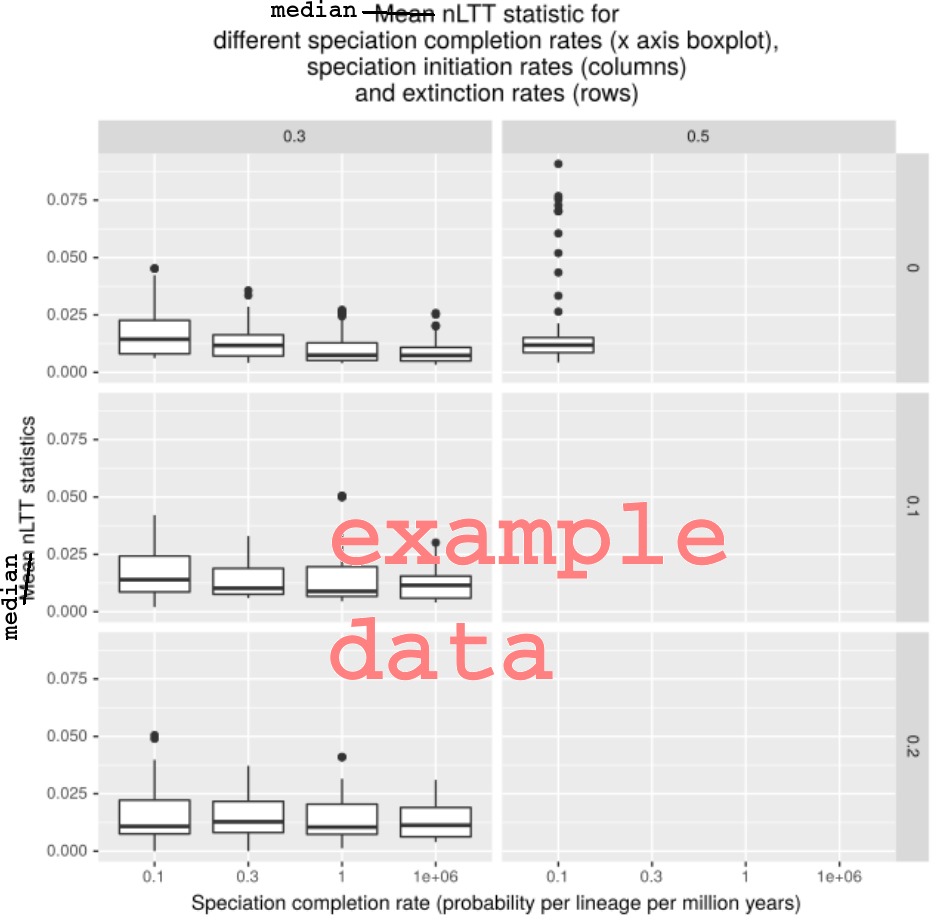
\includegraphics[width=0.8\textwidth]{fig_nltt_stats_per_setup.png}
  \caption{
    nLTT statistic distribution per biological parameter set, using the
    balanced data set
  }
\end{figure}

\begin{figure}[!htbp]
  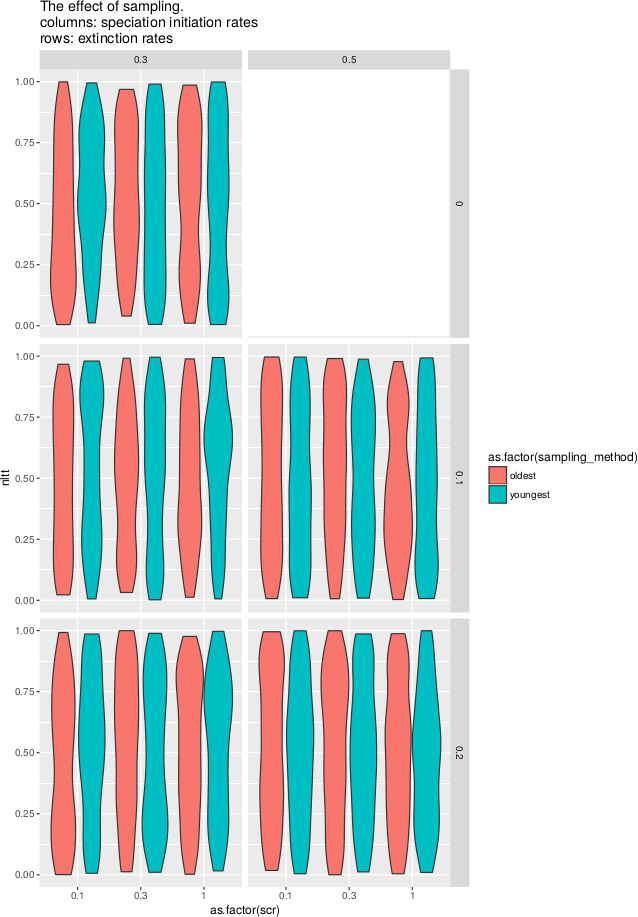
\includegraphics[width=0.8\textwidth]{fig_sampling.png}
  \caption{
    nLTT statistic distribution per biological parameter set per sampling
    regime, using the data set conditioned on sampling regime having an effect 
  }
\end{figure}

%%%%%%%%%%%%%%%%%%%%%%%%%%%%%%%%%%%%%%%%%%%%%%%%%%%%%%%%%%%%%%%%%%%%%%%%%%%%%%%%%%%%%%
\section{Glossary}
%%%%%%%%%%%%%%%%%%%%%%%%%%%%%%%%%%%%%%%%%%%%%%%%%%%%%%%%%%%%%%%%%%%%%%%%%%%%%%%%%%%%%%

% Please supply, as a separate list, the definitions of field-specific terms used in your article.

%%%%%%%%%%%%%%%%%%%%%%%%%%%%%%%%%%%%%%%%%%%%%%%%%%%%%%%%%%%%%%%%%%%%%%%%%%%%%%%%%%%%%%
\section{Acknowledgements}
%%%%%%%%%%%%%%%%%%%%%%%%%%%%%%%%%%%%%%%%%%%%%%%%%%%%%%%%%%%%%%%%%%%%%%%%%%%%%%%%%%%%%%

We would like to thank the Center for Information Technology of the University of Groningen for their support
and for providing access to the Peregrine high performance computing cluster.

%%%%%%%%%%%%%%%%%%%%%%%%%%%%%%%%%%%%%%%%%%%%%%%%%%%%%%%%%%%%%%%%%%%%%%%%%%%%%%%%%%%%%%
\section{Authors' contributions}
%%%%%%%%%%%%%%%%%%%%%%%%%%%%%%%%%%%%%%%%%%%%%%%%%%%%%%%%%%%%%%%%%%%%%%%%%%%%%%%%%%%%%%

RJCB and RSE conceived the idea for this experiment and package. 
RJCB created and tested the experiment and package, 
and wrote the first draft of the manuscript. 
RSE contributed substantially to revisions.

% Bibliography
%%%%%%%%%%%%%%%%%%%%%%%%%%%%%%%%%%%%%%%%%%%%%%%%%%%%%%%%%%%%%%%%%%%%%%%%%%%%%%%%%%%%%%
% MEE style
\bibliographystyle{mee}
\bibliography{article}
%%%%%%%%%%%%%%%%%%%%%%%%%%%%%%%%%%%%%%%%%%%%%%%%%%%%%%%%%%%%%%%%%%%%%%%%%%%%%%%%%%%%%%

%%%%%%%%%%%%%%%%%%%%%%%%%%%%%%%%%%%%%%%%%%%%%%%%%%%%%%%%%%%%%%%%%%%%%%%%%%%%%%%%%%%%%%
\appendix
%%%%%%%%%%%%%%%%%%%%%%%%%%%%%%%%%%%%%%%%%%%%%%%%%%%%%%%%%%%%%%%%%%%%%%%%%%%%%%%%%%%%%%

%%%%%%%%%%%%%%%%%%%%%%%%%%%%%%%%%%%%%%%%%%%%%%%%%%%%%%%%%%%%%%%%%%%%%%%%%%%%%%%%
\begin{table}
  \centering 
  \begin{tabular}{l l l}
    \hline
    Parameter             & Description & Values \\
    \hline
    \hline
    $b = b_g = b_i$       & Speciation initiation rate & 0.1, 0.5, 1.0 \\
    $\lambda$             & Speciation completion rate & 0.1, 0.3, 1.0, $\infty$ \\
    $\mu = \mu_g = \mu_i$ & Extinction rate & 0.0, 0.1, 0.2, 0.4 \\
    \hline
    $t_c$                 & Crown age & 15 \\
    $\sigma_c$            & Standard deviation around crown age & 0.001 \\
    $M$                   & Sampling method & MRCA, MDCA or random \\
    $r$                   & Mutation rate & $\frac{1000}{15}$ \\
    $l_a$                 & DNA alignment length & $15K$ \\
    $f_i$                 & MCMC sampling interval & 1K or more \\
    $R_i$                 & RNG seed incipient tree & 1 to 40K \\
    $R_a$                 & RNG seed alignment simulation & $R_i$ \\
    $R_b$                 & RNG seed BEAST2 & $R_i$ \\
    \hline
  \end{tabular}
  \caption{
    Overview of the 12 simulation parameters. Above the horizontal line is 
    the biological parameter set. Sampling method $M$ is random for the general
    data set. For the data set exploring the effect of sampling, MRCA is
    used for odd values of $R_i$, and MDCA is used for even values of $R_i$.
    $R_i$ is 1 for the first simulation, 2 for the next, etcetera.
  }
  \label{table:parameters}
\end{table}
%%%%%%%%%%%%%%%%%%%%%%%%%%%%%%%%%%%%%%%%%%%%%%%%%%%%%%%%%%%%%%%%%%%%%%%%%%%%%%%%

%%%%%%%%%%%%%%%%%%%%%%%%%%%%%%%%%%%%%%%%%%%%%%%%%%%%%%%%%%%%%%%%%%%%%%%%%%%%%%%%
\begin{table}
  \centering 
  \begin{tabular}{l l}
    \hline
    $n$ & Description \\
    \hline
    \hline
    $12$   & simulation parameters, see table \ref{table:parameters} \\
    $1000$ & nLTT statistic values \\
    $11$ & ESSes of all parameters estimated by BEAST2 (see specs below) \\
    \hline
  \end{tabular}
  \caption{
    Specification of the data sets. $n$ denotes the number
    of columns a certain item will occupy, resulting in a table of 
    1023 columns and 40K rows.
  }
  \label{table:specs}
\end{table}
%%%%%%%%%%%%%%%%%%%%%%%%%%%%%%%%%%%%%%%%%%%%%%%%%%%%%%%%%%%%%%%%%%%%%%%%%%%%%%%%

%%%%%%%%%%%%%%%%%%%%%%%%%%%%%%%%%%%%%%%%%%%%%%%%%%%%%%%%%%%%%%%%%%%%%%%%%%%%%%%%
\begin{table}
  \centering 
  \begin{tabular}{l l}
    \hline
    \# & Description \\
    \hline
    \hline
    1 & posterior \\
    2 & likelihood \\
    3 & prior \\
    4 & treeLikelihood \\
    5 & TreeHeight \\
    6 & BirthDeath \\
    7 & BDBirthRate \\
    8 & BDDeathRate \\
    9 & logP.mrca \\
    10 & mrcatime \\
    11 & clockRate \\
    \hline
  \end{tabular}
  \caption{
    Overview of the 11 BEAST2 estimated parameters
  }
  \label{table:estimated_parameters}
\end{table}
%%%%%%%%%%%%%%%%%%%%%%%%%%%%%%%%%%%%%%%%%%%%%%%%%%%%%%%%%%%%%%%%%%%%%%%%%%%%%%%%

\end{document}
